\input{../header.tex}

\subject{VERSUCHSNUMMER 503}
\title{Der Millikan-Öltröpfchenversuch}
\date{
  Durchführung: 02.05.2023
  \hspace{3em}
  Abgabe: 07.05.2023
}

\begin{document}

\maketitle
\thispagestyle{empty}
\tableofcontents
\newpage
\setcounter{page}{1}
\section{Ziel}
\label{sec:Ziel}
Durch diesen Versuch soll die Elementarladung $e_0$ und weiter die Avogadokonstante $A_{\text{A}}$ bestimmt werden.
\section{Theorie}
\label{sec:Theorie}

Die Elementarladungen kann man durch den sogenannten Millikan-Versuch bestimmen. Dazu müssen kleine Öltröpfchen 
in das vertikale Feld eines Plattenkondensators gebracht werden. Durch Reibung erhalten diese eine elektrische Ladung und folglich 
erfahren sie eine Kraft bedingt durch das E-Feld. Auf das Tröpfchen wirken dann insgesamt 4 Kräfte, welche in \autoref{fig:Kräfte} schematisch dargestellt sind.
\begin{figure}
    \centering
    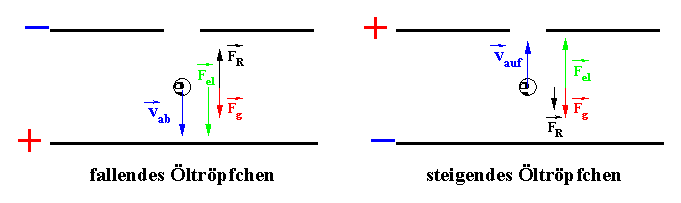
\includegraphics{Kräfte.pdf}
    \caption{Darstellung der auf das Öltröpfchen wirkende Kräfte \cite{ap503}.}
    \label{fig:Kräfte}
\end{figure}
Die einzelnen Kräfte werden durch folgende Formeln beschrieben
\begin{align*}
    \vec{F_{\text{g}}} &=m\vec{g}\quad (\text{Gewichtskraft}),\\
    \vec{F_{\text{R}}} &=6\pi r \eta_{\text{L}} \vec{v}\quad (\text{Reibungskraft}),\\
    \vec{F_{\text{el}}}&=q\cdot \vec{E}\quad (\text{Kraft durch das E-Feld}) ,\\
    \vec{F_{\text{a}}} &=m_{\text{L}}\cdot g\quad (\symup{Auftriebskraft}).
\end{align*}
Hierbei ist $m$ die Masse des Tröpfchens, $\vec{g}$ die Erdbeschleunigung, $r$ der Radius des Tröpfchens, $\eta_{\text{L}}$ die Viskosität der Luft,
$\vec{v}$ die Geschwindigkeit, $q$ die Ladung, $E$ das E-Feld des Plattenkondensators und $m_{\text{L}}$ die Masse der durch das Tröpfchen verdrängten Luft.
Bei ausgeschaltetem E-Feld kann dann, wenn die Gleichgewichtsgeschwindigkeit des Tröpfchens $\vec{v_0}$ erreicht ist ein Kräftegleichgewicht aufgestellt werden
\begin{align*}
    \vec{F_{\text{g}}}-\vec{F_{\text{a}}}&= \vec{F_{\text{R}}}\. ,\\
    \frac{4\pi}{3}r^3(\rho_{\text{Öl}}-\rho_{\text{L}})g&= 6\pi r \eta_{\text{L}} \vec{v}\. .
\end{align*} 
Nach Umstellen folgt so für den Radius des Tröpfchen
\begin{equation}
    r=\sqrt{\frac{9\eta_{\text{L}}v_0}{2g(\rho_{\text{Öl}}-\rho_{\text{L}})}}
    \label{eqn:r1}
\end{equation}
Wenn nun eine Spannung angelegt wird, steigt oder sinkt das Tröpfchen. Für die Richtung spielt die Polung des Kondensators eine große Rolle (siehe \autoref{fig:Kräfte}).
Wirkt die elektrische Kraft nach unten, erhöht sich die Sinkgeschwindigkeit und die Kräftegleichung erweitert sich zu
\begin{equation*}
    \frac{4 \pi}{3} r^3\left(\rho_{Öl}-\rho_L\right) g-6 \pi \eta_L r v_{ab}=-q E\. .
\end{equation*}
Wenn das Tröpfchen steigt, ergibt sich die Kräftegleichung zu
\begin{equation*}
    \frac{4 \pi}{3} r^3\left(\rho_{Öl}-\rho_L\right) g+6 \pi \eta_L r v_{auf}=+q E\. .
\end{equation*}
Aus diesen beiden Gleichungen lässt sich nun die Ladung des Tröpfchens über die Formel 
\begin{equation}
    q=3 \pi \eta_L \sqrt{\frac{9}{4} \frac{\eta_L}{g} \frac{\left(v_{a b}-v_{a u f}\right)}{\left(\rho_{O e l}-\rho_L\right)}} \cdot \frac{\left(v_{a b}+v_{a u f}\right)}{E}
  \label{eqn:q}
\end{equation}
und der Tröpfchenradius 
\begin{equation*}
    r=\sqrt{\frac{9}{4} \frac{\eta_L}{g} \frac{\left(v_{a b}-v_{a u f}\right)}{\left(\rho_{O e l}-\rho_L\right)}}
    \label{eqn:r2}
\end{equation*}
bestimmt werden.
Da die Tröpfchen kleiner sind als die mittlere freie Weglänge in Luft $\vec{l}$, muss die Viskosität $\eta_{\text{L}}$ der Luft über die Gleichung
\begin{equation*}
    \eta_{\text{eff}}=\eta_{\text{L}}\left(\frac{1}{1+A\frac{1}{r}}\right)=\eta_{\text{L}}\left(\frac{1}{1+B\frac{1}{pr}}\right)
\end{equation*}
ermittelt werden. Die Größe $B=6.17\cdot 10^{-3} \text{ Torr}\cdot \unit{\cm}$ ist der Cunningham-Korrekturterm.
Da die mittlere freie Weglänge $\vec{l}$ umgekehrt proportional zum Luftdruck $p$ ist, ist die korrigierte Ladung
\begin{equation}
    q^{\frac{2}{3}}_{korrigiert}= q^{\frac{2}{3}}_0\left(1+B\frac{1}{pr}\right)\. .
    \label{eqn:qeff}
\end{equation}
\section{Aufbau}
\label{sec:Aufbau}

Die Messapparatur des Millikanversuches ist in \autoref{fig:aufbau} abgebildet.

\begin{figure}
    \centering
    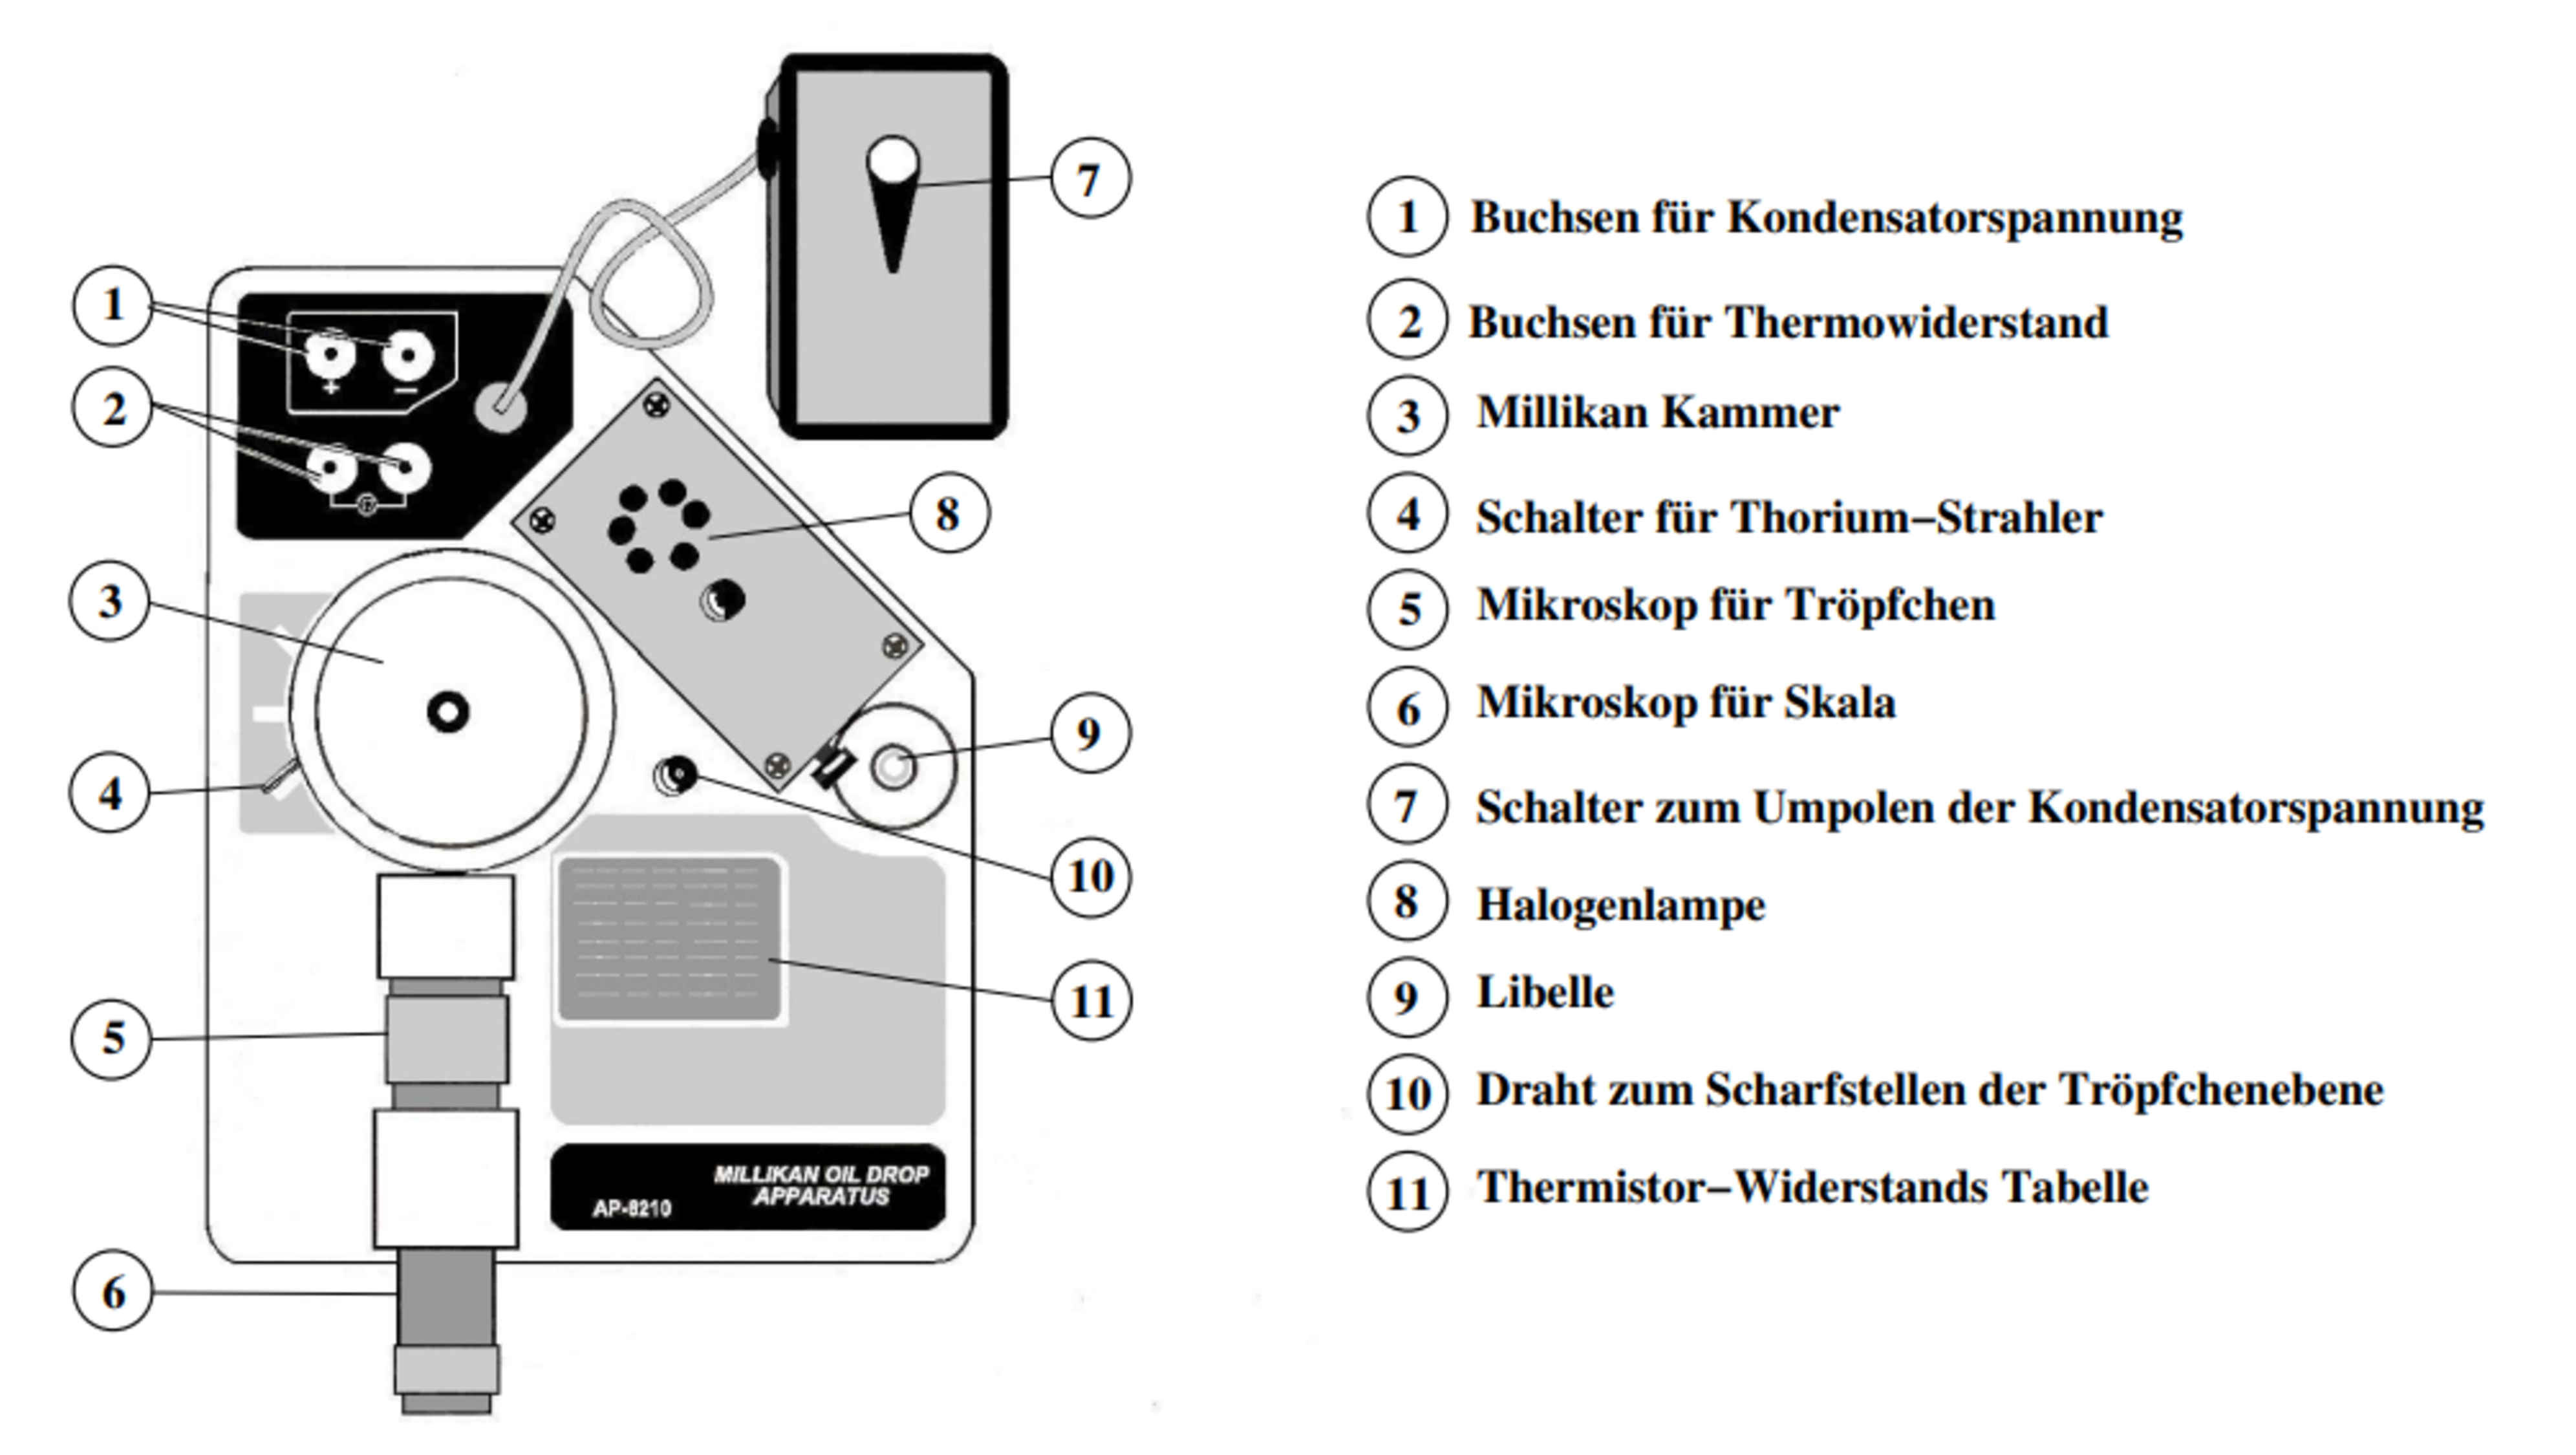
\includegraphics[height = 9cm]{Aufbau.pdf}
    \caption{Aufbau des Millikan-Öltröpfchenversuchs \cite{ap503}.}
    \label{fig:aufbau}
\end{figure}

Dieser besteht aus einer Kammer, die einen Plattenkondensator enthält. Dessen Platten 
haben einen Abstand von $d = (7.6250 \pm 0.0051) \,\unit{\milli\meter}$. Die obere
Platte hat in der Mitte eine Öffnung, durch die die mittels eines Zerstäubers 
entstandenen Öltröpfchen in den Plattenkondensator gelangen. Die Öltröpfchen, welche 
mit einer Halogenlampe angestrahlt werden, können
dann mit einem Mikroskop beobachtet werden.

Mittels des Thermowiderstands wird während der Messung die Temperatur überprüft, da sich
diese durch die Halogenlampe erhöht. Desweiteren kann die Ladung der 
Öltröpfchen durch ein radioaktives $\alpha$-Präparat verändert werden. Das Präparat 
selbst kann abgeschirmt oder aktiviert werden. 
\section{Durchführung}
\label{sec:Durchführung}

Vor Beginn des Versuchs muss mit Hilfe der Libelle überprüft werden, ob die Messapparatur 
waagerecht steht. Außerdem wird kontrolliert, ob die Spannungsquelle am Plattenkondensator 
anliegt.

Zuerst müssen bei abgeschaltetem Plattenkondensator Öltröpfchen in die Kammer gesprüht 
werden. Dabei ist wichtig, dass nicht zu viel Öl in die Kammer gelangt. Nun wird 
ein relativ langsames Öltröpfchen ausgewählt, welches im Anschluss über eine selbst 
gewählte Strecke beobachtet wird. Vor dessen Untersuchung, muss überprüft werden, ob das 
Tröpfchen geladen ist. Dies geschieht, indem man das elektrische Feld eingeschaltet 
wird und einmal umgelegt wird. Wenn es bei dem umgepolten Feld keine Veränderung gegenüber 
vorher gibt, ist das Teilchen ungeladen. In diesem Fall muss bei ausgeschaltetem 
Feld, das radioaktive Präparat aktiviert werden, um das Tröpfchen entsprechend zu 
laden. 

Jetzt wird mit der eigentlichen Messung begonnen. Dazu wird die Fallgeschwindigkeit $v_{\symup{ab}}$
des Tröpfchens gemessen, indem die Zeit gemessen wird, in der das Tröpfchen 
eine bestimmte Strecke zurücklegt. Dann wird das Feld umgepolt und die 
Steiggeschwindigkeit $v_{\symup{auf}}$ gemessen. Diese Messung wird bei dem selben 
Tröpfchen so oft wie möglich wiederholt. Zuletzt wird die Gleichgewichtsgeschwindigkeit 
$v_0$ bei ausgeschaltetem elektrischen Feld gemessen. 

Die gesamte Messung wird für mehrere Öltröpfchen wiederholt. Außerdem werden für insgesamt 
fünf verschiedene Kondensatorspannungen jeweils mehrere Öltröpfchen beobachtet.
Dabei darf die Spannung an den Kondensatorplatten $500\,\unit{\volt}$ nicht übersteigen.
\section{Auswertung}
\label{sec:Auswertung}

\subsection{Fehlerrechnung}
\label{sec:Fehlerrechnung}
Für die Fehlerrechnung werden folgende Formeln aus der Vorlesung verwendet.
für den Mittelwert gilt
\begin{equation}
    \overline{x}=\frac{1}{N}\sum_{i=1}^N x_i ß\; \;\text{mit der Anzahl N und den Messwerten x} 
    \label{eqn:Mittelwert}
\end{equation}
Der Fehler für den Mittelwert lässt sich gemäß
\begin{equation}
    \increment \overline{x}=\frac{1}{\sqrt{N}}\sqrt{\frac{1}{N-1}\sum_{i=1}^N(x_i-\overline{x})^2}
    \label{eqn:FehlerMittelwert}
\end{equation}
berechnen.
Wenn im weiteren Verlauf der Berechnung mit der fehlerhaften Größe gerechnet wird, kann der Fehler der folgenden Größe
mittels Gaußscher Fehlerfortpflanzung berechnet werden. Die Formel hierfür ist
\begin{equation}
    \increment f= \sqrt{\sum_{i=1}^N\left(\frac{\partial f}{\partial x_i}\right)^2\cdot(\increment x_i)^2}.
    \label{eqn:GaussMittelwert}
\end{equation}


\subsection{Tröpfchengeschwindigkeiten}
Für zwei verschiedene Spannungen wurde sowohl im eingeschalteten elektrischen Feld die Auf- und Abstiegszeit des jeweiligen Tröpfchens und bei ausgeschaltetem 
Feld die Zeit der Gleichgewichtsgeschwindigkeit gemessen. Für eine Spannung von $U = 201\,\unit{\volt}$ sind die Messdaten der einzelnen 
Tröpfchen in \autoref{tab:200} dargestellt, für eine Spannung von $U = 250\,\unit{\volt}$ in \autoref{tab:250}. Die Messwerte, die mit einem 
Sternchen markiert wurden, wurden in den handschriftlichen Messdaten falsch aufgeschrieben (siehe Anhang).

\begin{table}
    \centering
    \caption{Messdaten der Auf- und Abstiegszeit bei $U=201\,\unit{\V}$.}
\begin{tabular}{c c c c}
    \toprule
        Tröpfchen &$t_{\symup{auf}} \mathbin{/} \unit{\s}$ & $t_{\symup{ab}}\mathbin{/} \unit{\s}$ & $t_0 \mathbin{/}\unit{\s}$ \\
    \midrule
    1&7.19&3.29&12.57\\
    &8.02&3.65&\\
    &7.91&4.51&\\
    2&3.00&2.97&37.04\\
    &3.19&3.05&\\
    &3.28&1.02&\\
    3&1.43&1.24&73.73\\
    &1.60&1.10&\\
    &1.18&1.38&\\
    4&1.28&1.00&72.05\\
    &1.11&1.28&\\
    &1.47&1.30&\\
    5&5.38&2.06&26.80\\
    &1.95&2.32&\\
    &3.50&3.17&\\
    6&1.82&2.80&62.36\\
    &7.80&2.18&\\
    &8.50&2.94&\\
    7&3.72&9.29&31.75\\
    &4.11&8.29&\\
    &3.24*&14.39*&\\
    8&6.77&8.21&20.41 \\
    &10.65&8.51&\\
    &12.86&5.81&\\
    9&2.04*&1.50*&72.52\\
    &2.13&1.78&\\
    &2.33&1.97&\\
    10&2.06&1.62&73.85 \\
    &1.99&1.79&\\
    &2.45&1.78& \\
    \bottomrule
    \end{tabular}
    \label{tab:200}
\end{table}

\begin{table}
    \centering
    \caption{Messdaten der Auf- und Abstiegszeit bei $U=250\,\unit{\V}$.}
\begin{tabular}{c c c c}
    \toprule
        Tröpfchen &$t_{\symup{auf}} \mathbin{/} \unit{\s}$ & $t_{\symup{ab}}\mathbin{/} \unit{\s}$ & $t_0 \mathbin{/}\unit{\s}$ \\
    \midrule
    1&1.88&1.51&92.45 \\
    &5.67&1.82& \\
    &2.35&5.06& \\
2&4.99&5.17&105.44 \\
    &5.06&4.62& \\
    &3.19&4.57& \\
  3&4.98&4.93&/ \\
     &5.79&4.40& \\
    &4.69&4.08& \\
4&8.85&4.55&21.89 \\
    &8.19&4.94& \\
     &8.50&4.93& \\
  5&4.88&5.47&/ \\
     &5.25&5.90& \\
    &5.03&5.43& \\
6&11.88&7.72&48.65 \\
   &10.59&8.43& \\
    &9.89&7.82& \\
    \bottomrule
    \end{tabular}
    \label{tab:250}
\end{table}

\newpage
Nun werden die Abstiegs- und Aufstiegsgeschwindigkeiten sowie die Gleichgewichtsgeschwindigkeit $v_0$ mittels
\begin{equation*}
    v=\frac{s}{t}
\end{equation*} 
berechnet. Dabei ist $s=0.5\,\unit{\milli\m}$. Des Weiteren werden die Geschwindigkeiten $v_{\symup{auf}}$ und $v_{\symup{ab}}$ für jeden Tropfen gemittelt und dann
dessen Differenz $\bar{v}_{\symup{ab}}-\bar{v}_{\symup{auf}}$ betrachtet. Alle Werte werden in \autoref{tab:200geschw} dargestellt. 
Die Differenz $\bar{v}_{\symup{ab}}-\bar{v}_{\symup{auf}}$ wird durch die Relation
\begin{equation}
    \bar{v}_{\symup{ab}}-\bar{v}_{\symup{auf}} = 2v_0
    \label{eqn:gültigkeit}
\end{equation}
mit der Gleichgewichtsgeschwindigkeit verglichen.
Um sich auf einen Bereich einzuschränken, werden alle Werte, die die Relation 
\begin{equation*}
    0.5\leq \frac{2v_0}{\bar{v}_{\text{auf}}-\bar{v}_{\text{ab}}}\leq 1.5
\end{equation*}
erfüllen, als auswertbar angenommen.

\begin{sidewaystable}
    \centering
    \caption{Messdaten der Auf- und Abstiegsgeschwindigkeit bei $U=201\,\unit{\V}$.}
\begin{tabular}{c c c c c c c c}
    \toprule
        Tröpfchen &$v_{\symup{auf}} \mathbin{/} 10^{-3}\unit{\m\per\s}$ & $v_{\symup{ab}}\mathbin{/} 10^{-3}\unit{\m\per\s}$ & $\bar{v}_{\symup{auf}} \mathbin{/} 10^{-3}\unit{\m\per\s}$& $\bar{v}_{\symup{ab}} \mathbin{/} 10^{-3}\unit{\m\per\s}$ & $\bar{v}_{\symup{ab}} -\bar{v}_{\symup{ab}} \mathbin{/} 10^{-3}\unit{\m\per\s}$ & $v_0 \mathbin{/}10^{-3}\unit{\m\per\s}$ & $2v_0 \mathbin{/}10^{-3}\unit{\m\per\s}$\\
    \midrule
    1&0.0695&0.1520&0.0650&0.1333&0.0682&0.0398&0.0796\\
    &0.0623&0.1370&&&&& \\
    &0.0632&0.1109&&&&& \\
2&0.1667&0.1684&0.1586&0.2742&0.1155&0.0135&0.0270\\
    &0.1567&0.1639&&&&& \\
    &0.1524&0.4902&&&&& \\
3&0.3497&0.4032&0.3620&0.4067&0.0447&0.0068&0.0136\\
    &0.3125&0.4545&&&&& \\
    &0.4237&0.3623&&&&& \\
4&0.3906&0.5000&0.3937&0.4251&0.0313&0.0069&0.0139\\
    &0.4505&0.3906&&&&& \\
    &0.3401&0.3846&&&&& \\
5&0.0929&0.2427&0.1641&0.2053&0.0413&0.0187&0.0373\\
    &0.2564&0.2155&&&&& \\
    &0.1429&0.1577&&&&& \\
6&0.2747&0.1786&0.1326&0.1927&0.0601&0.0080&0.0160\\
    &0.0641&0.2294&&&&& \\
    &0.0588&0.1701&&&&& \\
7&0.0538&0.1344&0.0496&0.1368&0.0872&0.0157&0.0315 \\
    &0.0603&0.1217&&&&& \\
   &0.0347&0.1543&&&&& \\
8&0.0739&0.0609&0.0532&0.0686&0.0153&0.0245&0.0490 \\
    &0.0469&0.0588&&&&&\\
    &0.0389&0.0861&&&&&\\
9&0.2451&0.3333&0.2315&0.2893&0.0579&0.0069&0.0138\\
    &0.2347&0.2809&&&&&\\
    &0.2146&0.2538&&&&&\\
10&0.2427&0.3086&0.2327&0.2896&0.0569&0.0068&0.0135\\
    &0.2513&0.2793&&&&&\\
    &0.2041&0.2809&&&&&\\
    \bottomrule
    \end{tabular}
    \label{tab:200geschw}
\end{sidewaystable}

Von den gültigen Tröpfchen wird nun mittels \autoref{eqn:r2} der Tröpfchenradius berechnet. Dabei wird die temperaturabhängige Viskosität von Luft benötigt, dessen Werte 
in \autoref{tab:Viskositaet} aufgetragen sind. Für die Dichte von Luft wird $\rho_{\symup{L}} = 1.024 \,\unit{\kg\per\m^3}$ \cite{luftdichte} 
und für die Dichte von Öl wird $\rho_{\symup{Öl}} = 886 \,\unit{\kg\per\m^3}$ \cite{ap503} angenommen.



\begin{sidewaystable}
    \centering
    \caption{Messdaten der Auf- und Abstiegsgeschwindigkeit bei $U=250\,\unit{\V}$.}
\begin{tabular}{c c c c c c c c}
    \toprule
        Tröpfchen &$v_{\symup{auf}} \mathbin{/} 10^{-3}\unit{\m\per\s}$ & $v_{\symup{ab}}\mathbin{/} 10^{-3}\unit{\m\per\s}$ & $\bar{v}_{\symup{auf}} \mathbin{/} 10^{-3}\unit{\m\per\s}$& $\bar{v}_{\symup{ab}} \mathbin{/} 10^{-3}\unit{\m\per\s}$ & $\bar{v}_{\symup{ab}} -\bar{v}_{\symup{ab}} \mathbin{/} 10^{-3}\unit{\m\per\s}$ & $v_0 \mathbin{/}10^{-3}\unit{\m\per\s}$ & $2v_0 \mathbin{/}10^{-3}\unit{\m\per\s}$\\
    \midrule
    11&0.2660&0.3311&0.1900&0.2350&0.0459&0.0054&0.0108 \\
              &0.0882&0.2747&&&&& \\
              &0.2128&0.0988&&&&& \\
    12&0.1002&0.0967&0.1028&0.1206&0.0178&0.0047&0.0095 \\
              &0.0988&0.1082&&&&& \\
              &0.1094&0.1567&&&&& \\
    13&0.1004&0.1014&0.0978&0.1125&0.0147& -- & --\\
              &0.0863&0.1136&&&&& \\
               &0.1066&0.1225&&&&& \\
    14&0.0565&0.1099&0.0587&0.1042&0.0454&0.0228&0.0457 \\
              &0.0611&0.1012&&&&& \\
              &0.0588&0.1014&&&&& \\
    15&0.0914&0.1025&0.0894&0.0990&0.0096& --& -- \\
              &0.0847&0.0952&&&&& \\
              &0.0921&0.0994&&&&& \\
    16&0.0421&0.0648&0.0466&0.0627&0.0161&0.0103&0.0206 \\
              &0.0472&0.0593&&&&& \\
            &0.0506&0.0639&&&&& \\
    \bottomrule
    \end{tabular}
    \label{tab:2500geschw}
\end{sidewaystable}
\begin{table}
    \centering
    \caption{Lufttemperaturen und Luftviskositäten \cite{ap503}.}
\begin{tabular}{c c c}
    \toprule
        $R\mathbin{/}\unit{\mega\ohm}$ &$T\mathbin{/}\unit{\celsius}$ & $\eta_{\symup{L}}\mathbin{/}10^{-5}\symup{Nsm^{-2}}$ \\
    \midrule
    2.05 & 24.0 & 1.844 \\
    2.08 & 23.5 & 1.840\\
    2.17 & 22.0 & 1.834\\
    2.20 & 21.5 & 1.832\\
     \bottomrule
    \end{tabular}
    \label{tab:Viskositaet}
\end{table}

Damit berechnen sich die Radien zu
\begin{align*}
    r_1 &= 1.6723 \cdot 10^{-7} \,\unit{\m} \; ,\\
    r_5 &= 2.9967 \cdot 10^{-7} \,\unit{\m}\; .
\end{align*}
Als Fehlerabweichung wird dabei für die Zeit $\symup{\Delta} t = 0.01\,\unit{\sec}$ und für die Strecke $\symup{\Delta}s = 0.02\,\unit{\mm}$.

Für die zweite Messreihe mit einer Kondensatorspannung von $250\, \unit{\volt}$ war es teilweise nicht möglich eine Gleichgewichtsgeschwindigkeit $v_0$ zu bestimmen, da die Tröpfchen sich ohne E-Feld nicht bewegt haben.
Aus der zweiten Messreihe sind somit nur 2 Werte, die die Relation aus \autoref{eqn:gültigkeit} erfüllen.
Die weiteren Berechnungen sind somit nur mit Daten dieser Tropfen valide.
%Nach \autoref{eqn:r2} ergeben sich die Radien der beiden Tröpfchen zu 
%\begin{align*}
%    r_{14}& = 1.4764\cdot 10^{-5}\, \unit{\meter}\\
%    r_{16}& = 9.9231\cdot 10^{-6}\, \unit{\meter}\. .
%\end{align*}
Das Bestimmen des Radius ist über \autoref{eqn:r2} möglich.
Somit folgen für die Radien 
\begin{align*}
    r_{14}& = 1.4748\cdot 10^{-7}\, \unit{\meter}\\
    r_{16}& =  5.1558\cdot 10^{-7}\, \unit{\meter}\. .
\end{align*}

Dabei wurde ein Luftdruck von $1.013\,\unit{\milli\bar}$ verwendet \cite{ap503}.

Die Ladungen der jeweiligen Tröpfchen berechnen sich mittels \autoref{eqn:q} zu und werden in \autoref{tab:q} dargestellt. Es wird ebenfalls die
korrigierte Ladung mittels \autoref{eqn:qeff} berechnet.
\begin{table}
    \centering
    \caption{Ladungen und korrigierte Ladungen.}
\begin{tabular}{c c c }
    \toprule
        Tröpfchen & $q \mathbin{/} 10^{-19}\unit{\coulomb}$ &$q_{\symup{korr}} \mathbin{/} 10^{-14}\unit{\coulomb}$  \\
    \midrule
    1& 12.183 \pm 0.008 & 22.059 \pm 0.015 \\
    5 & 7.117 \pm 0.005 & 10.198 \pm 0.007 \\
    14 & 4.0269 \pm 0.003 & 7.776 \pm 0.005 \\
    16 & 56.11 \pm 0.04 & 69.88 \pm 0.05 \\
    \bottomrule
    \end{tabular}
    \label{tab:q}
\end{table}

In \autoref{fig:ladungkorr} werden nun zur Bestimmung der Elementarladung die korrigierten Ladungen aufgetragen.
\begin{figure}
    \centering
    \includegraphics[height = 12cm]{build/Ladung.pdf}
    \caption{Korrigierte Ladungen.}
    \label{fig:ladungkorr}
\end{figure}
Die Ladungen wurden ihrer Größe nach sortiert und so zugeteilt, dass eine lineare Ausgleichskurve
\begin{equation*}
    y = mx + b
\end{equation*}
durch diese gelegt werden kann.
Die Parameter ergeben sich zu 
\begin{align*}
    m &=  \\
    b &=   \; . \\
\end{align*}
Nach zunächst groben Sortieren folgte die genauere Einordnung der Ladungen in ein Vielfaches von dem größten gemeinsamen Teiler, welcher dann dem Wert der gesuchten Elementarladung $e_0$ entspricht.
Die Steigung $m$ dieser Ausgleichsgerade entspricht demnach der gesuchten Größe.
Der graphisch bestimmte Wert für die Elementarladung liegt bei $e_0=2.417\cdot 10^{-19}\,\unit{\coulomb}$ und entspricht somit nicht ganz dem theoretischen Wert ($e_{0,\text{theo}}=1.602\cdot 10^{-19}\,\unit{\coulomb}$ \cite{e}), 
welcher ebenfalls in \autoref{fig:ladungkorr} mit einer Gerade dargestellt ist.

Die Avogadro-Konstante wird über die Formel 
\begin{equation*}
    N_{\text{A}}=\frac{F}{e_0} 
\end{equation*}
wobei F die Faraday-Konstante mit einem Wert $9.648\cdot 10^4\, \unit{\frac{\coulomb}{\mol}}$ ist, bestimmt.
Aus der oben bestimmten Ladung folgt so die Avogadro-Konstante
\begin{equation*}
    N_{\text{A,exp}}=\frac{F}{2.417\cdot 10^{-19}\,\unit{\coulomb}}= 3.992\cdot 10^{23}\, \unit{\mol}^{-1}
\end{equation*}

\section{Diskussion}
\label{sec:Diskussion}

Wenn der unkorrigierte Wert der Elementarladung mit dem Literaturwert verglichen wird, lässt sich eine Abweichung von $3.00 \,\%$ erkennen. Die
experimentell bestimmte Elementarladung stimmt im Rahmen der angegebenen Messunsicherheit mit dem theoretischen Wert überein. Jedoch befinden sich nach der
Korrektur zwei Ladungen unterhalb der Elementarladung, was so eigentlich nicht vorkommen dürfte. Dies kann aus Messfehlern resultieren. Gerade die Reaktionszeit beim Messen der Zeit hat einen großen Einfluss auf die Messdaten, gerade weil
das zu messende Zeitintervall teilweise sehr gering war. Desweiteren war es bei vielen Tropfen im Bild teilweise nur schwierig möglich, den gewählten 
Tropfen über mehrere Zeitintervalle nicht aus den Augen zu verlieren, sodass nicht auszuschließen ist, dass bei einer Messung verschiedene Tropfen 
gemessen wurden. Insgesamt gab es nur fünf Tropfen, die die nötige Bedingung erfüllten, sodass das Ergebnis statistisch noch nicht wirklich aussagekräftig ist.

Die experimentell bestimmte Avogadrokonstante weicht um $2.86\,\%$ von dem Literaturwert $N_{\symup{A}}=6.0221 \cdot10^{23} \,\symup{\frac{1}{mol}}$ 
\cite{avo} ab, stimmt aber ebenfalls im Rahmen der angegebenen Messunsicherheit überein.

\newpage
\printbibliography
\nocite{ap503}
\nocite{matplotlib}
\nocite{numpy}
\nocite{scipy}
\nocite{uncertainties}
\nocite{reback2020pandas}

\newpage
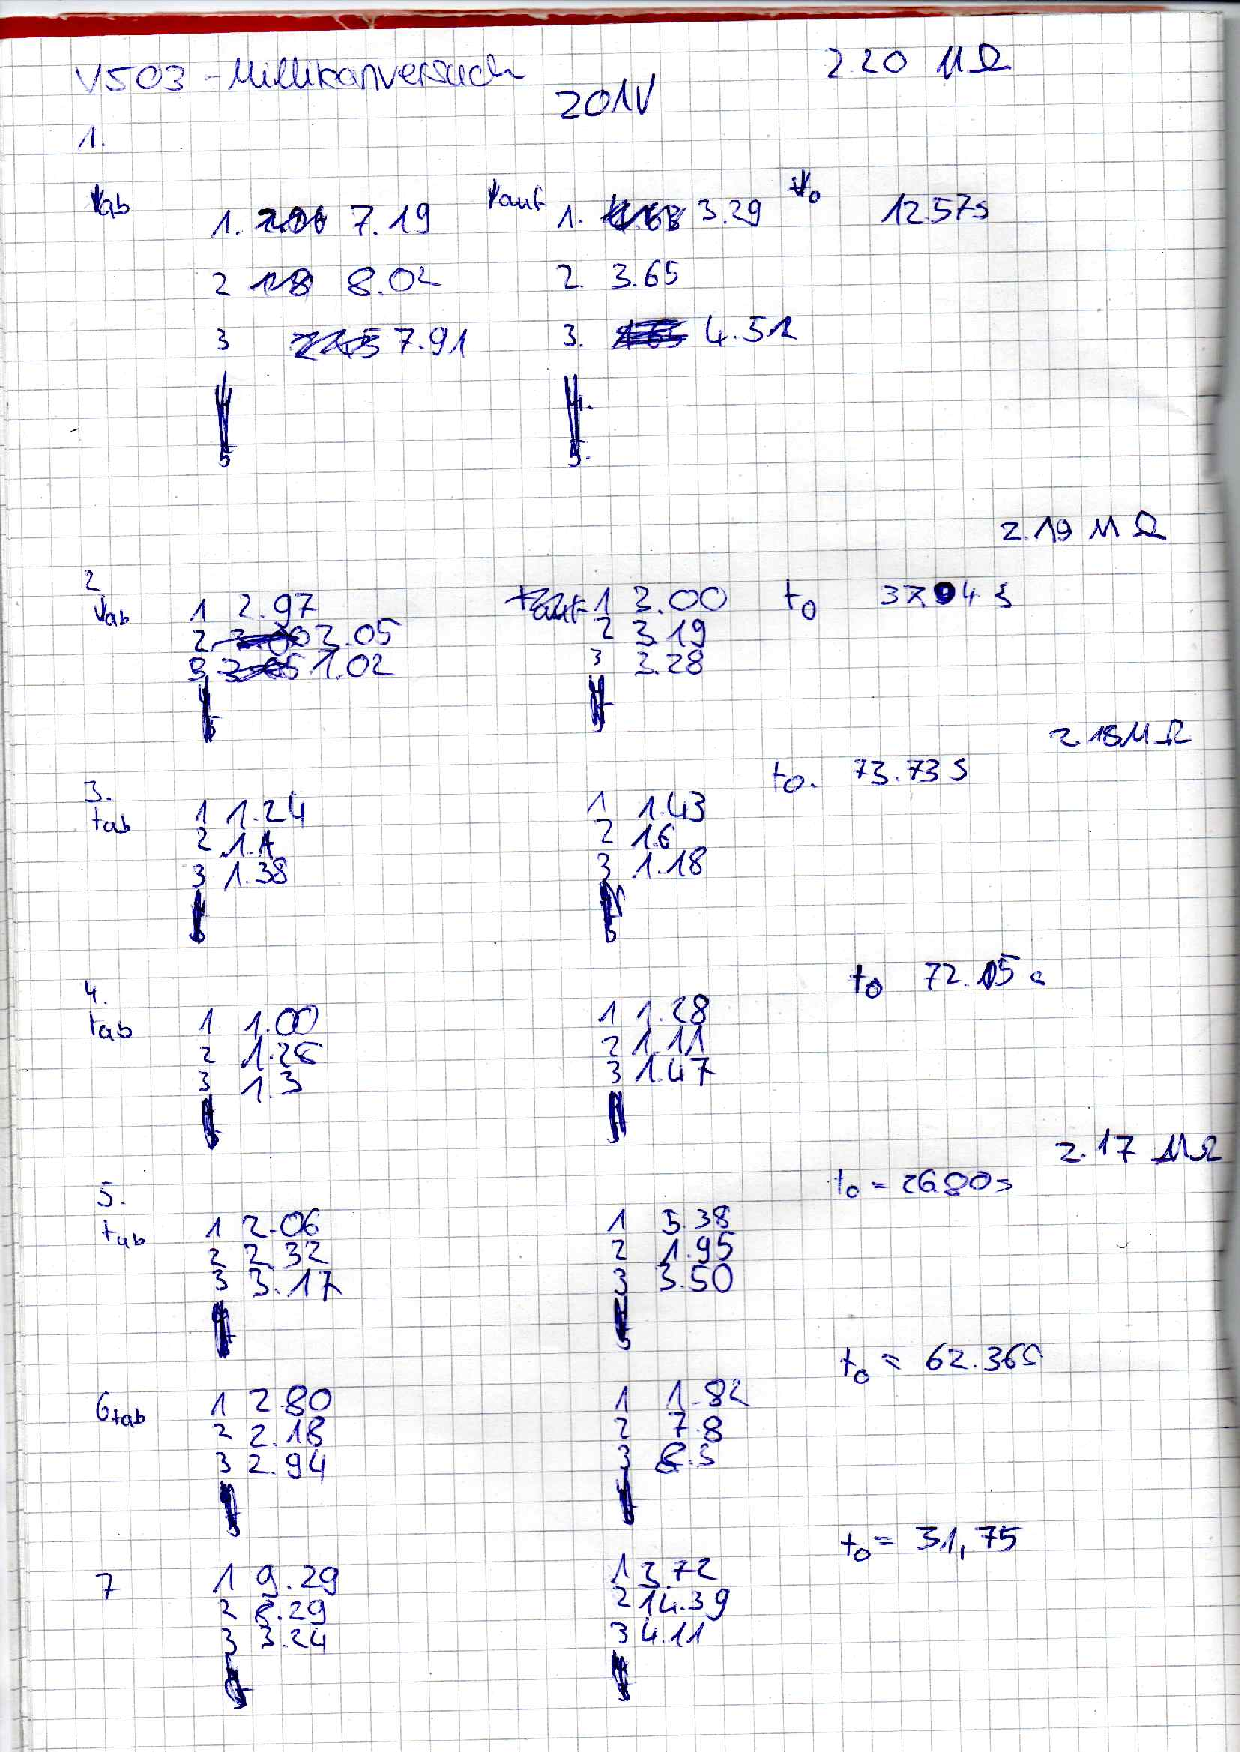
\includepdf[scale=0.7,pages=1,pagecommand=\section*{Anhang}\thispagestyle{empty}]{messdaten1.pdf}
\addcontentsline{toc}{section}{\protect\numberline{}Anhang}
%\includepdf[scale=0.9,pages=2-]{messdaten.pdf}
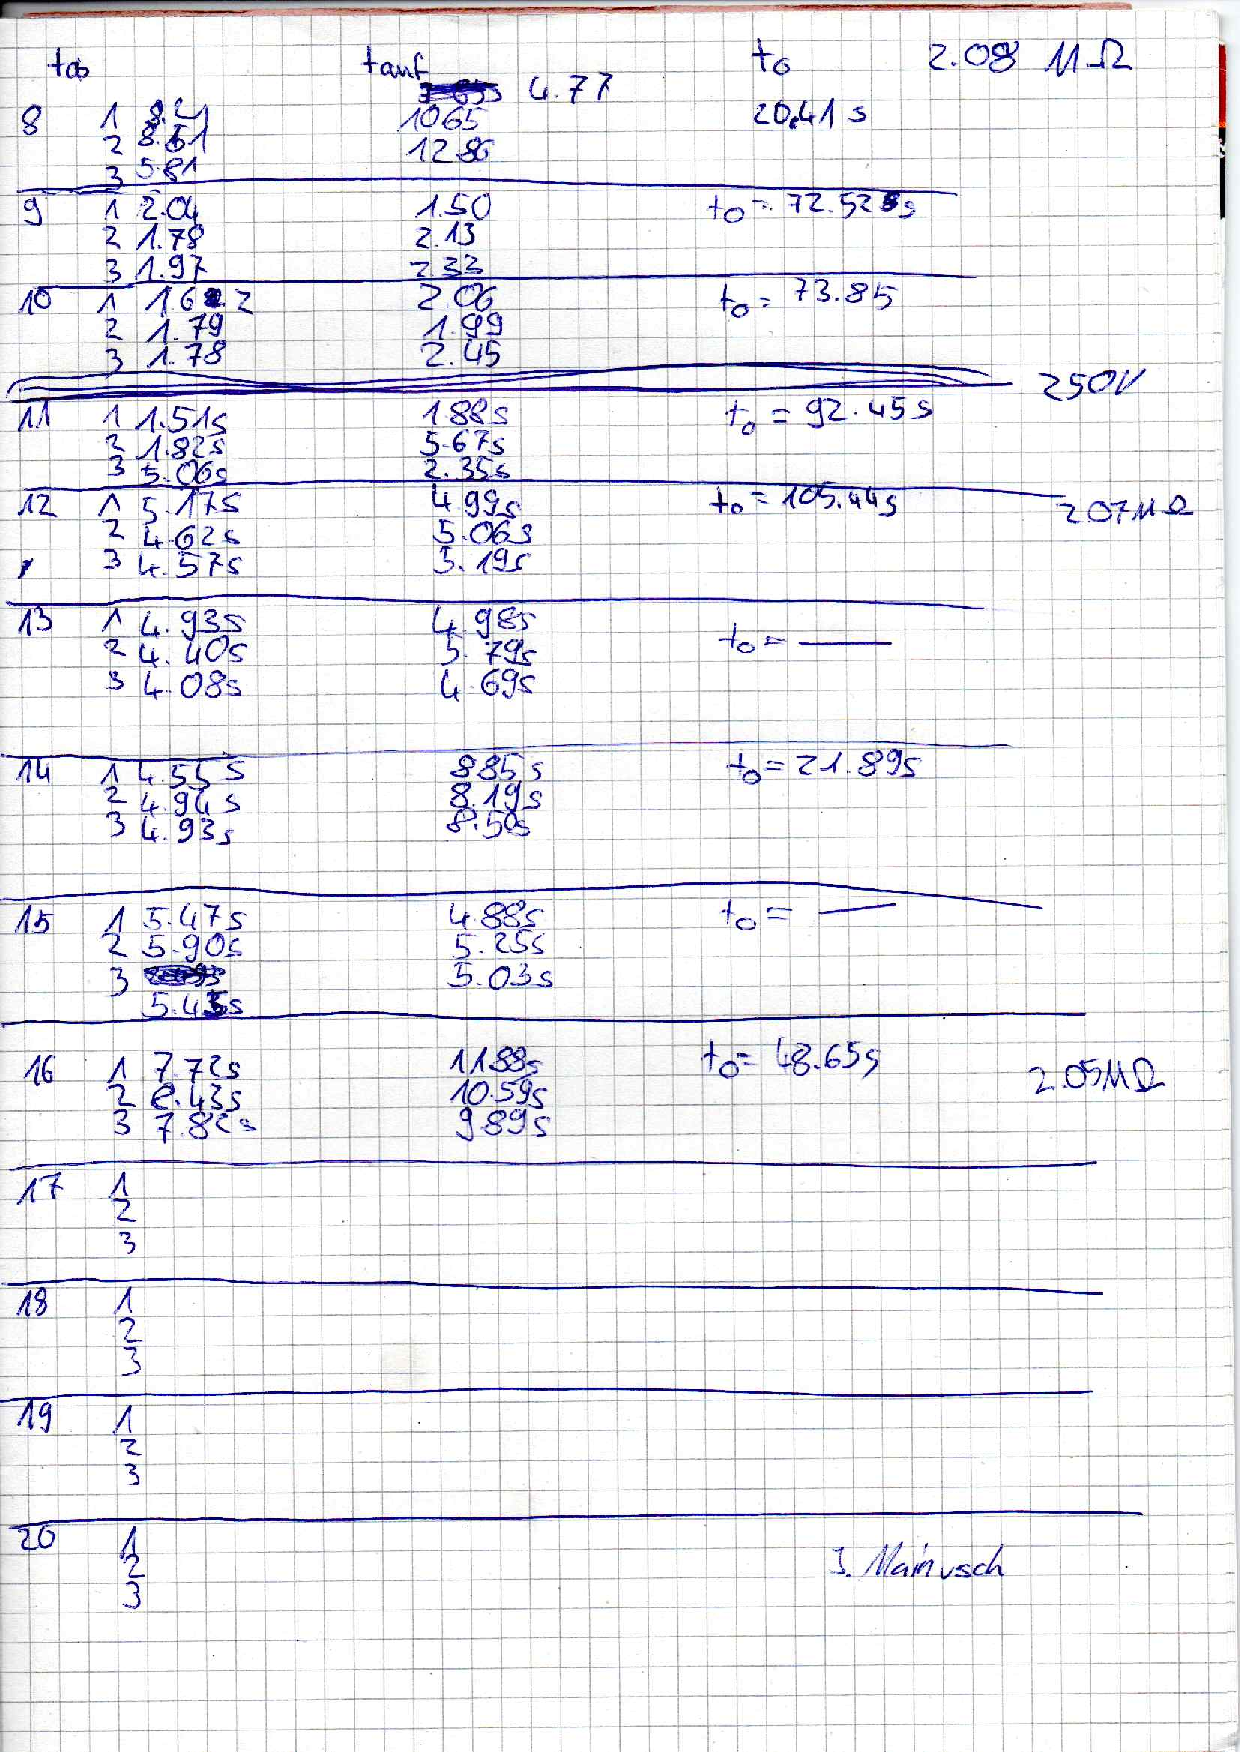
\includepdf[scale=0.7,pages=-]{messdaten2.pdf}

\end{document}
